\chapter{Multi-task learning}
Multi-task learning is a generalization of Transfer Learning to training a single model where the goal is to optimize for multiple objectives. 
Training a Multi-task model requires a set of distinct tasks to be posed as a Multi-task learning problem.
It can have many benefits when applied correctly, such as making the models more general by regularization and reducing computational requirements.
On the other hand, if Multi-task learning is applied to problems that don't train well in a Multi-task setting, the resulting models can be significantly worse than the Single-task counterparts.

\section{Definition}
Multi-task learning is quite similar to Transfer learning. 
However, the main difference lies in the fact that the goal is to generalize to solve and improve performance in all tasks using some shared representation. 
In contrast, Transfer learning aims to optimize a single new task, ignoring the performance on the original entirely. 
Often the shared layers are initialized using some ImageNet model, and Transfer learning as the ImageNet backbone is an architectural feature shared in many models.

The formal definition for Multi-task learning follows the definition given in \citep{surveyOnMultiTask}. 
A learning problem consists of ${m}$ related learning tasks ${\{T_i\}_{i=1}^m}$ that are trained together. 
Each task has a dataset ${D_i}$ with ${n_i}$ pairs ${\{x_{j}^{i}, y_{j}^{i}\}_{j=1}^{n_i}}$, where ${x_{j}^{i}}$ refers to the input of task ${T_i}$ and ${y_{j}^{i}}$ is the label corresponding to the input vector.
Let ${X^i}$ = (${x_{1}^{i}, ... , x_{n_i}^{i})}$ be the input matrix for task ${T_i}$.
In a Multi-task setting there can be ${x}$ such that ${x \in X^i}$ and ${x \in X^j}$ or ${X^i = X^j}$ for some ${i \ne j}$, meaning that a single image has multiple labels or an entire data set has labels for multiple tasks.

To train the network, each task ${T_i}$ needs to have its loss function defined.
A commonly used way to get the total loss of the input by using the weighted loss functions for all tasks, resulting in a formula ${L_{total} = \sum_i{w_i L_i}}$, where ${L_i}$ is the loss function for task ${T_i}$ and ${w_i}$ is the weight that specifies the sensitivity of the task \citep{usingUncertaintyToWeighLosses}. 
The sensitivity of the tasks is an essential parameter to get right as choosing a too high parameter for some task might lead to a solution that is optimal for only the most sensitive task, starving the others \citep{whichTasks}.

Once the loss function is specified, the actual training is quite similar to training a Single-task model.
The one new thing to consider in a Multi-task setting is the sampling ratio of the different tasks as some tasks can be easier to learn or contain significantly more or less data compared to other tasks.

\section{Benefits}
Depending on how Multi-task learning is applied, it can provide a multitude of benefits to the model.
Many of these benefits stem from the fact that the model gets to see more data, and the various tasks can make it easier to find useful features.
Different kinds of data sets have different kinds of noise, learning multiple tasks makes it easier to distinguish which features are good and bad, some features may be difficult to learn on a dataset, but can be useful and borrowed from another and learning multiple tasks forces the model to not overfit on one of them \citep{ruderOverview}.

These benefits come up when the tasks are compatible and allow the model to learn more general features, generally leading to better performance on the distinct tasks. 
When the needed features between tasks are conflicting, the model performance tends to go down \citep{uberNet}.
The problem of deciding what to share is not easy to solve.

The benefits of Multi-task learning come up, especially when dealing with limited amounts of data, in which case, particularly finding the features that matter without overfitting can be complicated. 
For example \citep{biologicalMultitask} found that Multi-task learning could improve gene expression pattern classifiers when trained in a Multi-task setting. 
The Multi-task classifier was significantly better than the one only using Transfer learning, showing that the features learned were more general.

Another significant boon of Multi-task models, especially in embedded domains, is the reduction in model size and inference time. 
As many classifiers are dependent on an embedding of an image to produce results, using a shared embedding of an image for multiple tasks means that the model requires only a single partly or completely shared backbone. 
For example \citep{multiPoseNet} uses a shared backbone to detect people in an image and to detect keypoints on their body and then finally to do a semantic segmentation of the image while also improving performance on most of the tasks.

Finally, a model using Multi-task learning can take advantage of the different losses to produce a more optimal loss weighing strategy compared to constant weighting. 
Picking the weights in the total loss function is very important as with poor weights, the optimization can be difficult or even impossible \citep{lossWeighting}. 
The weights become even more critical if the losses for various tasks are different, for example, one task might use mean squared error as a loss function and another cross-entropy, and the resulting loss values might differ by orders of magnitude.
The total loss function can be modified by adding an uncertainty weighting to each of the tasks by considering the uncertainty of the prediction \citep{usingUncertaintyToWeighLosses}. 
Depending on the task, the benefit compared to an unweighted loss can be significant \citep{usingUncertaintyToWeighLosses} or, in some cases, only small \citep{lossWeighting}.

\section{Hard parameter sharing}
Show how multiple heads can be combined to produce outputs for various tasks using different heads, show results from sharing all/some layers. \citep{visualPerson} \citep{selfDriving} \citep{healthyDrink}

\section{Soft parameter sharing}

\begin{figure}[h!] 
\centering 
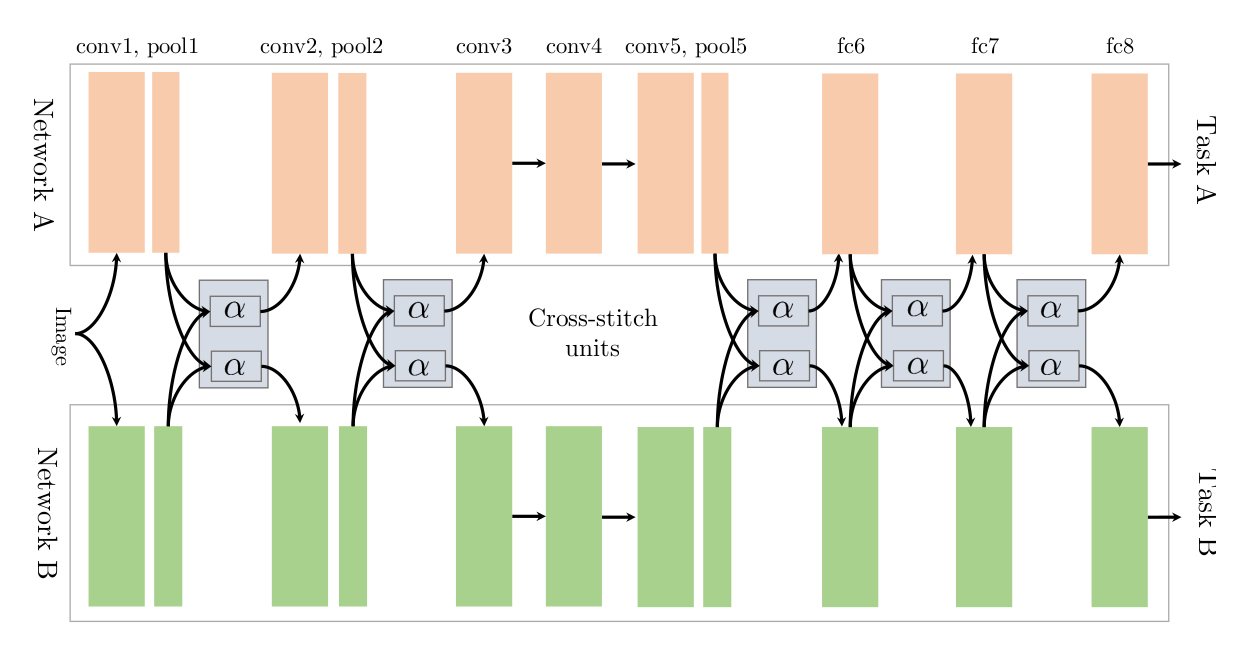
\includegraphics[width=0.8\textwidth]{imgs/stitch.png}
\caption{Cross-stitch architecture. Figure from \citep{crossStitch}.\label{fig:params}}
\end{figure}

Soft parameter sharing is quite similar to learning each task on their own since each task has separate weights. Soft parameter sharing happens by picking some layers, where some metric constrains the parameters to be similar, like ${l_2}$ distance \citep{ruderOverview}. 

The sharing functionality can be more complicated than just basic regularization. For example, the Cross-stitch units \citep{crossStitch} are a particular type of soft sharing, where the stitch units combine tasks A and B using a linear combination of the activations, visualized in Figure 3.1. The benefit here is that the user does not need to specify how much should be shared between the tasks, but it is rather learned in the cross-stitch unit. If nothing needs to be shared, then the network can learn to assign the weight for the other task to zero.

This kind of sharing does not scale very well as the number of tasks increases since calculating the relation between various tasks is quadratic. 
Since the joining logic requires extra parameters, it means there is even more to learn than just learning all the tasks separately. 
As soft sharing does not provide many of the benefits that are gained by hard sharing the parameters, it is not as popular, but still used in various cases.

\section{Special multi-task learning techniques}
Show how an attention layer can be added to augment the performance in various tasks in a multi-task setting \citep{multiTaskAttention}, specifically when the tasks are correlated \citep{multiTaskWeather} \citep{weatherNet}. Maybe some others as well.

\section{What and when to share}
What makes or breaks a Multi-task model is the decision on what should be shared, but determining what and how much should be shared is exponentially more expensive as the number of tasks grows. 
As experimentation is expensive, a good starting point is to try to find similar tasks that should do well together. 
However, there is no guarantee that even all the tasks within a single family of problems are beneficial for joint training, so some experimentation has to be done. 
The desired result in a Multi-task setting would be to share all the parameters between all the tasks, but as can be seen in \citep{uberNet}, that approach often significantly reduces performance.
If sharing an entire network does not produce good results, it can be a good idea only to share some part of it as the lower level features tend to be more general \citep{transferringMidLevelRepresentations}. 
By sharing only a part of the network, it may be possible to strike a good balance between performance and model complexity.

\begin{figure}[h!] 
\centering 
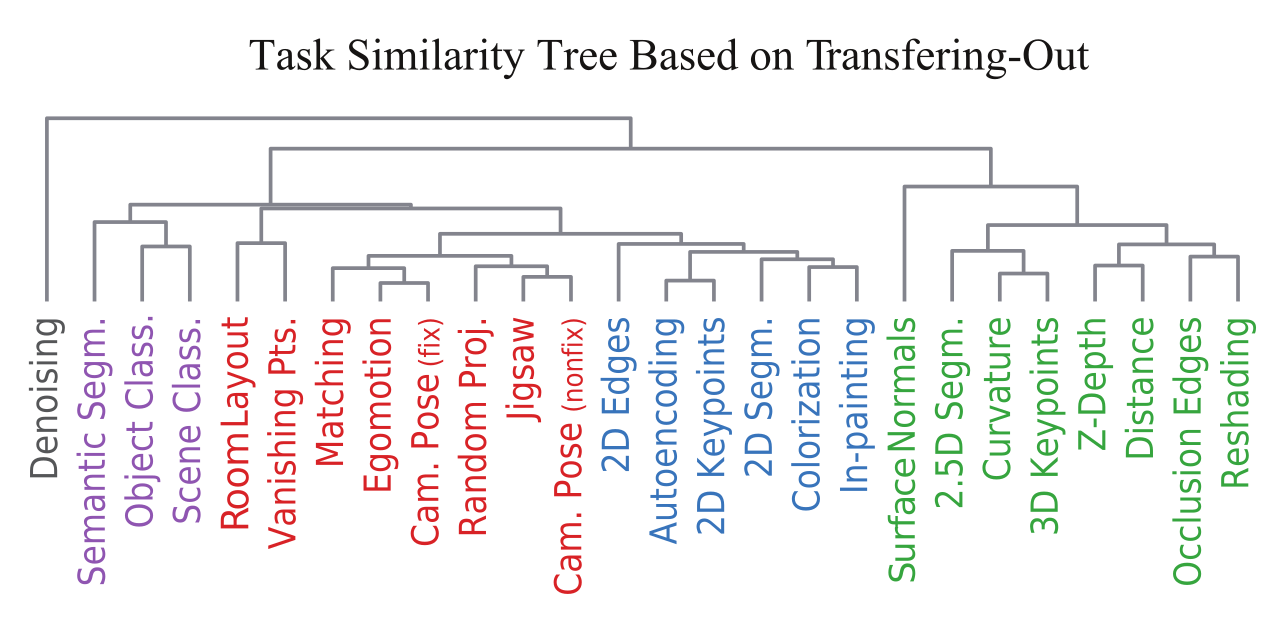
\includegraphics[width=0.8\textwidth]{imgs/taskonomy.png}
\caption{The taskonomy task similarity tree. Figure from \citep{taskonomy}.\label{fig:params}}
\end{figure}

An attempt to create a taxonomy of related tasks called Taskonomy to find out what tasks are beneficial for transfer learning exists in \citep{taskonomy}. 
The Taskonomy experiments pre-trained networks on tasks and then evaluated whether the features would transfer well to other tasks to end up with a hierarchical categorization of related tasks, shown in Figure 3.2. 
Still, the authors noted that, depending on model architecture and data set, the results could be different.

It would make sense that the results of the Taskonomy would be easily transferable to the Multi-task setting. 
When evaluating the Multi-task vs. Transfer affinity, it turns out that they are negatively correlated, at least in the case of the five tasks that were the focus of the experiments in \citep{whichTasks}. 
Based on this observation, it can be beneficial to train non-related tasks together. 
The authors suggest that the different tasks act as a good form of regularization. 
It could also be that some of the learned features work very well for the other task, but can't be easily learned with the dataset of the other task and vice versa.